\chapter{Pogojni stavek}

\section{Zakaj pogojni stavki?}

Vsi programi, ki smo jih do zdaj napisali (je bil mogoče samo eden?), so se izvedli po vnaprej določenem zaporedju. Od zgoraj navzdol so se namreč lepo po vrsti izvedli vsi stavki v programu. V določenih primerih pa bi posamezne stavke radi izvedli samo ob izpolnjenosti (ali pa neizpolnjenosti) izbranega pogoja. 

Poglejmo si spodnji primer:
\begin{zgled}
Napiši program, ki od uporabnika prebere telesno maso in višino in izpiše uporabnikov indeks telesne mase.
\end{zgled}
\begin{resitev}
Preko funkcije \texttt{input} bomo torej prebrali telesno maso in višino. Ker funkcija vrača niz, bomo obe vrednosti pretvorili v decimalno število (\texttt{float}). Potem bomo uporabili enačbo za izračun indeksa telesne mase: $itm = \frac{masa}{visina^2}$. Pri tem mora biti telesna masa podana v kilogramih, višina pa v metrih.
\begin{lstlisting}[language=Python,numbers=left]
masa = float(input("Vpiši svojo telesno maso [kg]: "))
visina = float(input("Vpiši svojo višino [m]: "))
itm = masa/visina**2
print("Tvoj ITM je", itm)
\end{lstlisting}
\end{resitev}

Zgornji program je popolnoma pravilen, bi ga pa radi še malo dopolnili. Veliko uporabnikov verjetno ne ve, kaj posamezna vrednost indeksa telesne mase (ITM) pomeni. Ali mora shujšati, je njegova telesena masa ustrezna, ali bi se moral malo zrediti? Če malo poenostavimo, lahko ljudi razdelimo v tri skupine, in sicer na tiste s premajhno telesno maso, tiste z ustrezno telesno maso in tiste s preveliko telesno maso:

\begin{tabular}{c|c}
     pogoj & skupina \\
     \hline
     ITM $<$ 18.5 & podhranjenost\\
     18.5 $\leq$ ITM $\leq$ 25 & normalna telesna masa\\
     25 $<$ ITM & debelost
\end{tabular}

\bigskip

Naš program bi torej radi dopolnili tako, da bo uporabniku izpisal tudi informacijo o tem, v katero skupino spada. Z drugimi besedami, če bo izpolnjen prvi pogoj (ITM $<$ 18.5), bi radi izpisali, da je uporabnik podhranjen, če bo izpolnjen drugi pogoj (18.5 $\leq$ ITM $\leq$ 25), da je njegova telesna masa ustrezna in če bo izpolnjen tretji pogoj (25 $<$ ITM), da je pretežak. Radi bi torej, da se določeni deli našega programa (v konkretnem primeru različni izpisi) izvedejo v odvisnosti od vrednosti ITM. 

\section{Osnovna oblika stavka \texttt{if}}

Za pisanje pogojnih stavkov bomo uporabili Pythonov stavek \texttt{if}. Njegova osnovna oblika je sledeča:
\begin{lstlisting}[language=Python]
if pogoj:
    # pogojni_stavki so zamaknjeni
    # pogojni stavki
    # če je pogoj izpolnjen
    ...
# skupni stavki
# ni več zamaknjeno
...
\end{lstlisting}
Začnemo torej z rezervirano besedico \textbf{\texttt{if}}, ki ji sledi pogoj. Temu sledi dvopičje (\texttt{:}), s katerim povemo, da je konec pogoja. Potem sledi pogojni del, ki se bo izvedel samo v primeru, da je podan pogoj izpolnjen. Pogojnemu delu sledijo stavki, ki se bodo izvedli v vsakem primeru, ne glede na izpolnjenost pogoja. Kako Pythonu povemo kje je konec pogojnega dela? Z zamikom \angl{indent}. Zgoraj smo tiste stavke, ki se izvedejo samo v primeru izpolnjenosti pogoja zamaknili, tako da smo pred njih vstavili tabulator (tipka \emph{Tab}) ali par presledkov (če smo natančni, se držimo dogovora štirih presledkov). Pogojni del smo zaključili tako, da smo enostavno nehali zamikati. Izvedbo zgornje kode prikazuje diagram poteka na sliki \ref{img:if1}.
\begin{figure}
    \centering
    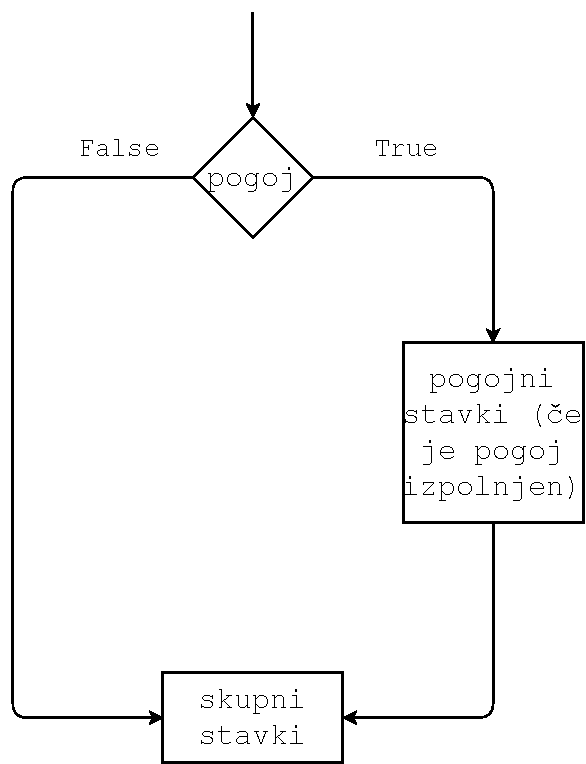
\includegraphics[width=0.5\linewidth]{img/if1.pdf}
    \caption{Diagram poteka osnovne oblike stavka \texttt{if}. V primeru, če je pogoj izpolnjen, se izvede pogojni del.}
    \label{img:if1}
\end{figure}

\section{Kaj je pogoj?}

Kaj pravzaprav predstavlja pogoj za izvedbo pogojnega dela stavka? Kot je razvidno iz slike \ref{img:if1} je pogoj nekaj, kar je lahko resnično \angl{true} ali neresnično \angl{false}. Pogoj moramo torej zastaviti kot vprašanje, na katerega lahko odgovorimo bodisi z odgovorom \emph{da} ali z odgovorom \emph{ne}. Pri formiranju vprašanja oziroma pogoja bomo torej večinoma uporabljali operatorje, ki vračajo take odgovore. Tem operatorjem pravimo \emph{pogojni operatorji}. Pa si poglejmo nekaj njihovih primerov.

\subsection{Primerjalni operatorji in podatkovni tip \texttt{bool}}

Prva skupina operatorjev, ki jih bomo uporabljali pri pisanju pogojev so t.i. \emph{primerjalni operatorji}, ki jih poznamo že iz matematike. To so npr. operator enakosti \texttt{==} (ker je enojni enačaj uporabljen za prirejanje, moramo za primerjanje uporabiti dvojni enačaj), operator neenakosti \texttt{!=}, večji \texttt{>}, večji ali enak \texttt{>=} itd. Poskusimo:
\begin{lstlisting}[language=Python]
>>> 1 == 1
True
>>> 1 == 2
False
>>> 1 != 2
True
>>> 1 > 2
False
>>> 1 <= 2
True
>>> 1 == 2.5
False
>>> 1 == 1.0
True
\end{lstlisting}
S primerjalnimi operatorji torej med seboj primerjamo dva podatka, rezultat primerjanja pa je bodisi vrednost \texttt{True} ali \texttt{False}. Rezultat primerjanja je podatek, ki lahko zavzame samo te dve vrednosti. Kakšen je podatkovni tip tega podatka?
\begin{lstlisting}[language=Python]
>>> type(True)
<class 'bool'>
>>> type(False)
<class 'bool'>
\end{lstlisting}
Za oblikovanje pogojev imamo torej na voljo poseben podatkovni tip, tj. \texttt{bool}, oziroma po angleško \emph{boolean}, ki lahko zavzame samo dve vrednosti, tj. \texttt{True} ali \texttt{False}. 

Poskusimo uporabo primerjalnih operatorjev v kombinaciji s pogojnim stavkom \texttt{if} uporabiti na zgledu iz začetka poglavja.
\begin{zgled}
Napiši program, ki od uporabnika prebere telesno maso in višino in izpiše uporabnikov indeks telesne mase (ITM). Poleg tega program uporabniku pove, v katero skupino spada. 
\end{zgled}
\begin{resitev}
Program od prej bomo dopolnili s pogojnim stavkom. Če je ITM manjši od 17.5, lahko program izpiše, da je uporabnikova telesna masa premajhna. Če je ITM večji od 25, lahko program izpiše, da je uporabnikova telesna masa prevelika. Kaj pa vmes? Tega pa zaenkrat še ne znamo. 
\begin{lstlisting}[language=Python,numbers=left]
masa = float(input("Vpiši svojo telesno maso [kg]: "))
visina = float(input("Vpiši svojo višino [m]: "))
itm = masa/visina**2
print("Tvoj ITM je", itm)
if ITM < 17.5:
    print("Tvoja telesna masa je premajhna")
if ITM > 25:
    print("Tvoja telesna masa je prevelika")
\end{lstlisting}
\end{resitev}

Primerjalne operatorje lahko uporabimo tudi nad podatki, ki niso števila.
\begin{lstlisting}[language=Python]
>>> "abc" == "abc"
True
>>> "abc" == "ABC"
False
>>> "abc" < "b"
True
>>> "abc" < "abc"
False
>>> "abc" < "abd"
True
\end{lstlisting}
Iz zgornjih zgledov vidimo tudi to, da Python loči med velikimi in malimi črkami in da so določeni nizi manjši od drugih. Kako pa primerjanje dveh nizov poteka? Na enak način, kot primerjamo nize, ko poskušamo besede sortirati po abecedi (npr. v slovarju ali telefonskem imeniku). Dve besedi primerjamo znak po znaku od začetka do konca, dokler ne pridemo do dveh znakov, ki se razlikujeta ali do konca ene izmed besed. Če se besedi ujemata po vseh znakih in je ena beseda krajša, je krajša beseda zagotovo manjša. Npr., beseda "beda" je manjša od besede "bedarija" (v slovarju bo beda nastopala pred bedarijo):
\begin{lstlisting}[language=Python]
>>> "beda" < "bedarija"
True
\end{lstlisting}
Beseda "bedno" pa ni manjša od besede "bedarija", čeprav je od nje krajša. Zakaj ne? Zato, ker se besedi razlikujeta v četrtem primerjanju na znakih "n" in "a" in ker "n" ni manjši od znaka "a".
\begin{lstlisting}[language=Python]
>>> "bedno" < "bedarija"
False
\end{lstlisting}
Takemu primerjanju pravimo \emph{leksikografsko} primerjanje. 

\subsection{Operatorja vsebovanosti}

Ko smo ravno pri nizih, lahko omenimo še \emph{operatorja vsebovanosti}, ki preverjata ali nekaj je (\texttt{in}) oziroma ni (\texttt{not in}) v posameznem nizu vsebovano. Operatorja bomo uporabljali tudi na drugih podatkovnih tipih, ki podobno kot nizi, vsebujejo druge podatke -- nizi so sestavljeni iz več znakov oziroma podnizov. Če je nek niz \texttt{podniz} vsebovan v nekem nizu \texttt{niz}, lahko preverim takole:
\begin{lstlisting}[language=Python]
>>> podniz in niz
\end{lstlisting}
Povadimo:
\begin{lstlisting}[language=Python]
>>> "beda" in "bedarija"
True
>>> "Beda" in "bedarija"
False
>>> "ana" in "anakonda"
True
>>> "ana" in "sanatorij"
True
>>> "a" in "abeceda"
True
\end{lstlisting}
Spet vidimo, da je znak \texttt{"b"} nekaj drugega kot znak \texttt{"B"} in da Python loči med malimi in velikimi črkami.

\subsection{Združevanje rezultatov primerjanja}

Pri reševanju naloge z izpisovanjem podatkov o ITM imamo še vedno težave s primerom, kjer morata biti izpolnjena dva pogoja hkrati (\texttt{ITM >= 18.5} in \texttt{ITM <= 25}). Končen pogoj za izvedbo izpisa \texttt{Tvoja telesna masa je ustrezna}, moramo torej sestaviti iz dveh pogojev. Za ta namen lahko uporabimo t.i. \emph{logične operatorje}, ki omogočajo medsebojno združevanje več spremenljivk tipa \texttt{bool}. Osnovna logična operatorja, ki ju bomo uporabljali v takem primeru sta operator \texttt{and} in operator \texttt{or}. Njuno delovanje lahko ponazorimo s spodnjo tabelo:

\begin{tabular}{cc|cc}
     \texttt{pogoj1} & \texttt{pogoj2}  & \texttt{pogoj1 and pogoj2} & \texttt{pogoj1 or pogoj2}\\
     \hline
     \texttt{False} & \texttt{False} & \texttt{False} & \texttt{False} \\
     \texttt{False} & \texttt{True} & \texttt{False} & \texttt{True} \\
     \texttt{True} & \texttt{False} & \texttt{False} & \texttt{True} \\
     \texttt{True} & \texttt{True} & \texttt{True} & \texttt{True} \\
\end{tabular}

\bigskip

Poglejmo si še en malo bolj konkreten primer:

\begin{tabular}{cc|cc}
     \texttt{17 >= 18.5} & \texttt{17 <= 25}  & \texttt{17 >= 18.5 and 17 <= 25} & \texttt{17 >= 18.5 or 17 <= 25}\\
     \hline
     \texttt{False} & \texttt{True} & \texttt{False} & \texttt{True} \\
\end{tabular}

\bigskip

V primeru, da morata biti izpolnjena oba vhodna pogoja, torej uporabimo operator \texttt{and}. Če je dovolj, da je izpolnjen samo eden izmed vhodnih pogojev, uporabimo operator \texttt{or}. Pogosto uporabljen logični operator je še operator \texttt{not}, ki \texttt{True} spremeni v \texttt{False} in obratno:
\begin{lstlisting}[language=Python]
>>> not True
False
>>> not False
True
>>> 17 >= 18.5
False
>>> not 17 >= 18.5
True
\end{lstlisting}

Zdaj lahko dokončamo zgled z izpisovanjem podatkov o ITM.
\begin{zgled}
Napiši program, ki od uporabnika prebere telesno maso in višino in izpiše uporabnikov indeks telesne mase (ITM). Poleg tega program uporabniku pove, v katero skupino spada. 
\end{zgled}
\begin{resitev}
Zdaj lahko dodamo še pogojni stavek, pri katerem bo pogoj sestavljen iz dveh delov. V tem primeru mora biti vrednost spremenljivke \texttt{ITM} večja ali enaka od 17.5 in manjša ali enaka od 25, kar lahko zapišemo s pogojem \texttt{17.5 <= ITM and ITM <= 25}.
\begin{lstlisting}[language=Python,numbers=left]
masa = float(input("Vpiši svojo telesno maso [kg]: "))
visina = float(input("Vpiši svojo višino [m]: "))
itm = masa/visina**2
print("Tvoj ITM je", itm)
if ITM < 17.5:
    print("Tvoja telesna masa je premajhna")
if ITM > 25:
    print("Tvoja telesna masa je prevelika")
if 17.5 <= ITM and ITM <= 25:
    print("Tvoja telesna masa je ustrezna")
\end{lstlisting}
\end{resitev}

Programiranja se učimo v jeziku Python med drugim tudi zato, ker ima kar nekaj uporabnih sladkorčkov (funkcionalnosti), ki jih drugi jeziki nimajo. Sestavljen pogoj \texttt{17.5 <= ITM and ITM <= 25} lahko v tem jeziku zapišemo tudi malo krajše, in sicer takole: \texttt{17.5 <= ITM <= 25}.

\section{Veja \texttt{else}}

Zgornji program je sicer pravilen, ni pa najlepši. V primeru, da je npr. izpolnjen prvi pogoj, tj. \texttt{ITM < 17.5}, ni nobene potrebe po tem, da preverjamo še izpolnjenost drugega in tretjega pogoja. To sicer v tem primeru ni narobe (lahko bi bilo), je pa nepotrebno in po eni strani naredi našo kodo manj pregledno, po drugi strani pa trati dragocen procesorski čas, saj preverja, če je določen pogoj izpolnjen, kljub temu, da vemo, da zagotovo ne more biti. Potek programa, ki smo ga napisali zgoraj, ponazarja slika \ref{img:if21}.

\begin{figure}
    \centering
    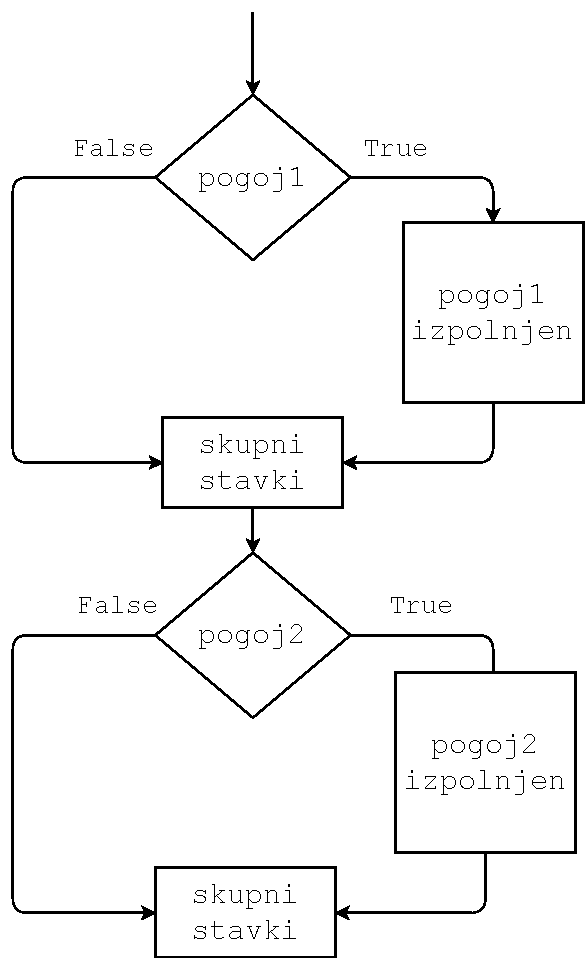
\includegraphics[width=0.5\linewidth]{img/if21.pdf}
    \caption{Izpolnjenost pogoja \texttt{pogoj2} se preverja ne glede na izpolnjenost pogoja \texttt{pogoj1}.}
    \label{img:if21}
\end{figure}

Do sedaj smo v primeru neizpolnjenosti pogoja vedno skočili na del \texttt{skupni stavki}, torej na del, ki se izvede neodvisno od izpolnjenost pogoja. V splošnem pa stavek \texttt{if} omogoča, da del kode izvedemo samo takrat, ko pogoj \textbf{ni} izpolnjen. To kodo podamo v veji \texttt{else} stavka \texttt{if}:
\begin{lstlisting}[language=Python]
if pogoj:
    # pogojni stavki
    # če je pogoj izpolnjen
    ...
else:
    # pogojni stavki
    # če pogoj ni izpolnjen
    ...
# skupni stavki
...
\end{lstlisting}
Potek izvajanja zgornje kode prikazuje slika \ref{img:if2}. 

\begin{figure}
    \centering
    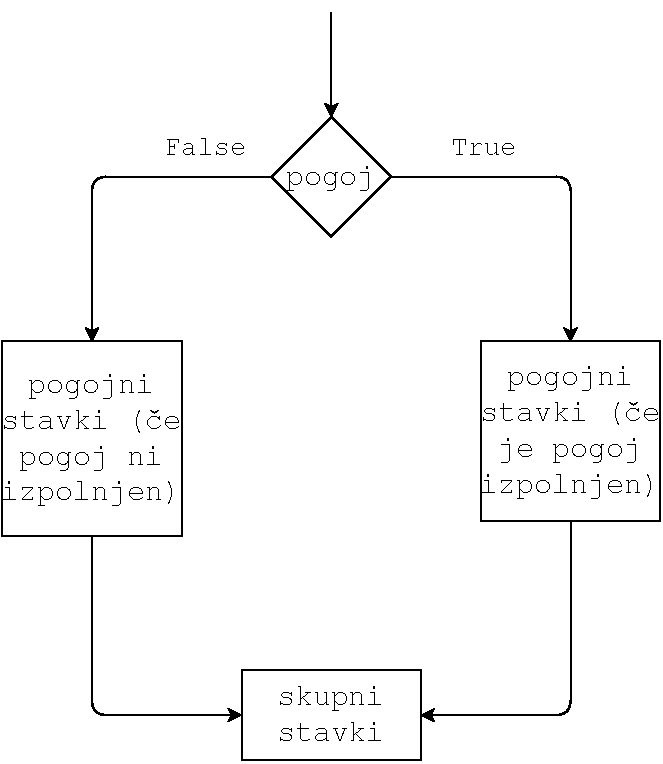
\includegraphics[width=0.5\linewidth]{img/if2.pdf}
    \caption{Dopolnitev stavka \texttt{if} z vejo \texttt{else}. Veja \texttt{else} se izvede samo v primeru, ko pogoj ni izpolnjen.}
    \label{img:if2}
\end{figure}

Uporabimo zgornji stavek za poenostavljeno rešitev naloge z izpisovanjem podatkov o ITM.
\begin{zgled}
Napiši program, ki od uporabnika prebere telesno maso in višino in izpiše uporabnikov indeks telesne mase (ITM). Poleg tega program uporabniku pove, če je njegova telesna masa ustrezna ali ne. 
\end{zgled}
\begin{resitev}
Tokrat bomo preverjali le pogoj o ustreznosti uporabnikove telesne mase. 
\begin{lstlisting}[language=Python,numbers=left]
masa = float(input("Vpiši svojo telesno maso [kg]: "))
visina = float(input("Vpiši svojo višino [m]: "))
itm = masa/visina**2
print("Tvoj ITM je", itm)
if 17.5 <= ITM <= 25:
    print("Tvoja telesna masa je ustrezna")
else:
    print("Tvoja telesna masa ni ustrezna")
\end{lstlisting}
\end{resitev}

\section{Veja \texttt{elif} in gnezdenje stavkov \texttt{if}}

Uporabnik zdaj ve, če je njegova telesna masa ustrezna. Če njegova telesna masa ni ustrezna, informacije o tem ali je pretežak ali prelahek nima (verjetno se mu to sicer dozdeva). Zgornji primer bi torej radi dopolnili tako, da znotraj veje \texttt{else} izvedemo dodatno primerjanje, na podlagi katerega bomo lahko ugotovili ali je ITM prevelik ali premajhen.

To lahko naredimo na dva načina. Elegantnejši način je uporaba stavka \texttt{elif}\footnote{Po slovensko bi lahko stavku \texttt{elif} rekli \emph{sicer pa, če velja}.}, ki omogoča preverjanje dodatnega pogoja znotraj veje \texttt{else}. Celoten stavek \texttt{if} z vejo \texttt{elif} zapišemo takole:
\begin{lstlisting}[language=Python]
if pogoj1:
    # pogojni stavki
    # pogoj1 izpolnjen
    ...
elif pogoj2:
    # pogojni stavki
    # pogoj1 ni izpolnjen
    # pogoj2 izpolnjen
    ...
else:
    # nobeden izmed pogojev
    # ni izpolnjen
# skupni stavki
...
\end{lstlisting}
V tem primeru se izpolnjenost pogoja \texttt{pogoj2} preverja samo, če pogoj \texttt{pogoj1} ni izpolnjen, veja \texttt{else} pa se izvede samo v primeru, ko ni bil izpolnjen nobeden izmed prejšnjih pogojev. Potek programa prikazuje slika \ref{img:if3}.

\begin{figure}
    \centering
    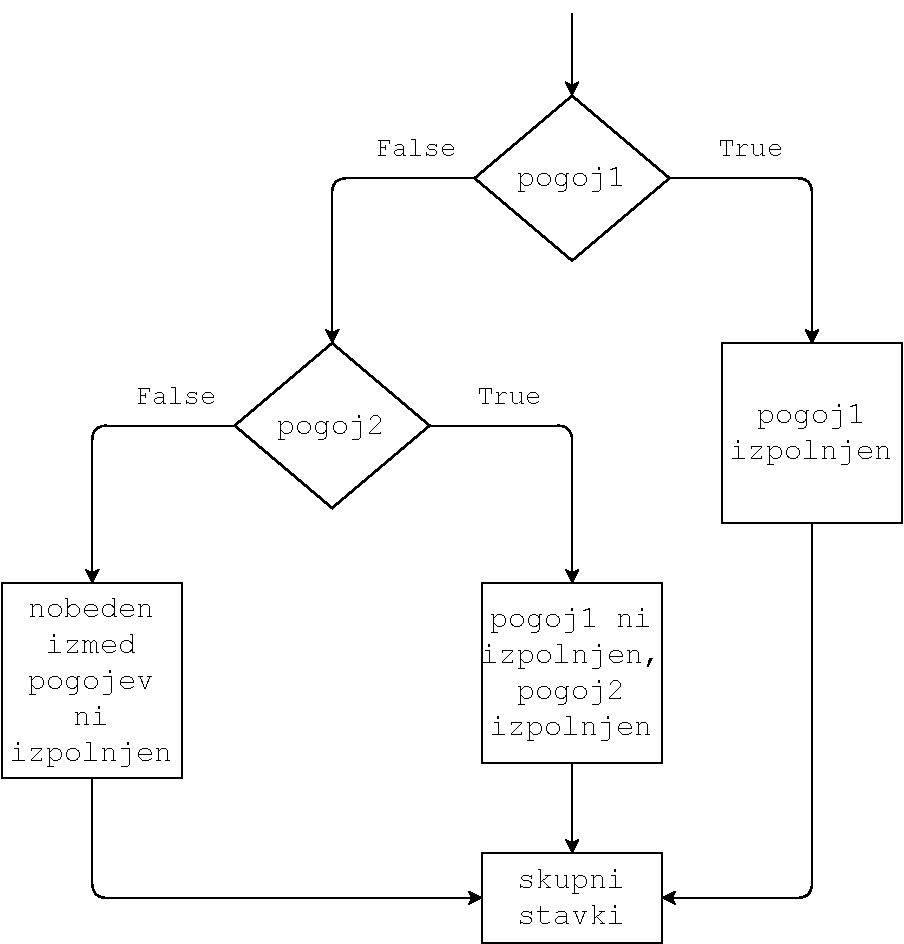
\includegraphics[width=0.65\linewidth]{img/if3.pdf}
    \caption{Dopolnitev stavka \texttt{if} z vejama \texttt{elif} in \texttt{else}. Veja \texttt{elif} se izvede samo v primeru, ko pogoj \texttt{pogoj1} ni izpolnjen, pogoj \texttt{pogoj2} pa je.}
    \label{img:if3}
\end{figure}

Zdaj lahko končno podamo lepšo rešitev zgleda z izpisovanjem podatkov o ITM.
\begin{zgled}
Napiši program, ki od uporabnika prebere telesno maso in višino in izpiše uporabnikov indeks telesne mase (ITM). Poleg tega program uporabniku pove, v katero skupino spada. 
\end{zgled}
\begin{resitev}
Najprej bomo preverili enega izmed pogojev, npr. če je ITM manjši od 17.5. V primeru, da je pogoj izpolnjen, izpišemo, da je telesna masa premajhna. V veji \texttt{elif} lahko preverimo naslednji pogoj, npr. če je ITM večji od 25. V primeru, da je izpolnjen ta pogoj, izpišemo, da je telesna masa prevelika. Če ni izpolnjen nobeden izmed obeh pogojev, lahko izpišemo, da je telesna masa ustrezna.
\begin{lstlisting}[language=Python,numbers=left]
masa = float(input("Vpiši svojo telesna masa [kg]: "))
visina = float(input("Vpiši svojo višino [m]: "))
itm = masa/visina**2
print("Tvoj ITM je", itm)
if ITM < 17.5:
    print("Tvoja telesna masa je premajhna")
elif ITM > 25:
    print("Tvoja telesna masa je prevelika")
else:
    print("Tvoja telesna masa je ustrezna")
\end{lstlisting}
\end{resitev}

Drug pristop k reševanju enakega problema je uporaba dodatnega stavka \texttt{if} znotraj veje \texttt{else}. Temu rečemo tudi \emph{gnezdenje} ali \emph{ugnezdeni stavek} \texttt{if}. Kodo bi napisali takole: \begin{lstlisting}[language=Python]
if pogoj1:
    # pogojni stavki
    # pogoj1 izpolnjen
    ...
else:
    if pogoj2:
        # tukaj so uporabljeni dvojni zamiki
        # pogojni stavki
        # pogoj1 ni izpolnjen
        # pogoj2 izpolnjen
        ...
    else:
        # tukaj so uporabljeni dvojni zamiki
        # nobeden izmed pogojev
        # ni izpolnjen
# skupni stavki
...
\end{lstlisting}
Začetek ugnezdenega stavka \texttt{if} je zamaknjen enkrat, s čimer povemo, da naj se izvede samo v primeru, ko pogoj \texttt{pogoj1} ni izpolnjen. Vsebino ugnezdenega stavka moramo zamakniti dvakrat. Izvedba zgornje kode bo enaka kot v primeru z uporabo veje \texttt{elif} in jo prikazuje slika \ref{img:if3}. 

Uporabimo ugnezden stavek \texttt{if} še pri reševanju naše naloge.
\begin{zgled}
Napiši program, ki od uporabnika prebere telesno maso in višino in izpiše uporabnikov indeks telesne mase (ITM). Poleg tega program uporabniku pove, v katero skupino spada. Uporabi ugnezden stavek \texttt{if}.
\end{zgled}
\begin{resitev}
Potek programa bo podoben kot prej za razliko od gnezdenja stavka \texttt{if}.
\begin{lstlisting}[language=Python,numbers=left]
masa = float(input("Vpiši svojo telesno maso [kg]: "))
visina = float(input("Vpiši svojo višino [m]: "))
itm = masa/visina**2
print("Tvoj ITM je", itm)
if ITM < 17.5:
    print("Tvoja telesna masa je premajhna")
else:
    if ITM > 25:
        print("Tvoja telesna masa je prevelika")
    else:
        print("Tvoja telesna masa je ustrezna")
\end{lstlisting}
\end{resitev}
